% !TeX root=../main.tex

\chapter*{پاسخ سوالات سری چهارم}
\section*{پاسخ سوال یک}

در این بخش، ابتدا کدی برای محاسبه ی ماتریس های تبدیل با در اختیار داشتن پارامتر های DH نوشته شده است. محاسبه ی ماتریس های تبدیل مربوط به هر یک از لینک ها با ساتفاده از تابع DH از پیش تعریف شده انجام گرفته است و برای سادگی کار، به جای فراخوانی مکرر این دستور با پارامتر های متفاوت برای هر لینک، ابتدا پارامترها در یک ماتریس تعریف شده و سپس در یک حلقه ی for، هر یک از ماتریس های تبدیل محاسبه می شوند. 
برای ربات $2R$ داریم:
\[
\text{$DH parameters$} = 
\left(\begin{array}{cccc}
	0 & 0 & a_1 & \theta_1 \\
	0 & 0 & a_2 & \theta_2
\end{array}\right)
\]
لازم به ذکر است که پیش از این، تعداد لینک ها برای برنامه مشخص شده است و همچنین، طول بازوهای ربات نیز در یک آرایه برای استفاده های بعدی تعریف شده است. 
ماتریس های تبدیل ربات $2R$ به صورت زیر محاسبه خواهند شد:
\[
T_{10} = 
\left(\begin{array}{cccc} 
	\cos \left(\theta_1 \right) & -\sin \left(\theta_1 \right) & 0 & 0\\
	\sin \left(\theta_1 \right) & \cos \left(\theta_1 \right) & 0 & 0\\
	0 & 0 & 1 & a_1 \\
	0 & 0 & 0 & 1
\end{array}\right)
\]

\[
T_{20} = 
\left(\begin{array}{cccc}
	\sigma_1  & -\cos \left(\theta_1 \right)\,\sin \left(\theta_2 \right)-\cos \left(\theta_2 \right)\,\sin \left(\theta_1 \right) & 0 & 0\\
	\cos \left(\theta_1 \right)\,\sin \left(\theta_2 \right)+\cos \left(\theta_2 \right)\,\sin \left(\theta_1 \right) & \sigma_1  & 0 & 0\\
	0 & 0 & 1 & a_1 +a_2 \\
	0 & 0 & 0 & 1
\end{array}\right)
\]

\[
\text{where} \quad \sigma_1 = \cos \left(\theta_1 \right)\,\cos \left(\theta_2 \right)-\sin \left(\theta_1 \right)\,\sin \left(\theta_2 \right)
\]

پس از محاسبه ی ماتریس های تبدیل برای هر لینک، می توان ماتریس های دوران و انتقال را در هر مفصل نسبت به دستگاه مختصات مرجع به سادگی به دست آورد. بنابراین، آخرین ماتریس دوران و انتقال به دست آمده، مربوط به پنجه ی ربات و یا نقطه ی $End Effector$ خواهد بود.
\[
P_{\text{$end effector$}} = 
\left(\begin{array}{c} 
	0\\
	0\\
	a_1 + a_2 
\end{array}\right)
\]

\[
R_{\text{$end effector$}} = 
\left(\begin{array}{ccc}
	\cos \left(\theta_1 \right)\,\cos \left(\theta_2 \right)-\sin \left(\theta_1 \right)\,\sin \left(\theta_2 \right) & -\cos \left(\theta_1 \right)\,\sin \left(\theta_2 \right)-\cos \left(\theta_2 \right)\,\sin \left(\theta_1 \right) & 0\\
	\cos \left(\theta_1 \right)\,\sin \left(\theta_2 \right)+\cos \left(\theta_2 \right)\,\sin \left(\theta_1 \right) & \cos \left(\theta_1 \right)\,\cos \left(\theta_2 \right)-\sin \left(\theta_1 \right)\,\sin \left(\theta_2 \right) & 0\\
	0 & 0 & 1
\end{array}\right)
\]

در گام بعد، ماتریس ژاکوبین محاسبه خواهد شد. اما نکته ای که باید در این قسمت به آن توجه شود این است که در این سوال، ماتریس های ژاکوبین مربوط به مرکز جرم هر لینک خواسته شده است و بنابراین، با توجه به محاسبات موجود در هر کتاب، برای لینک آخر باید نیمی از طول آن را در محاسبات لحاظ کرد و در ترم های قبلی، طول کامل بازوها را در نظر گرفت.

با توجه به این مورد، ابتدا در یک حلقه ی for، ماتریس های دوران و انتقال تجمعی برای مفاصل ربات به صورت کامل و بدون لحاظ کردن مراکز جرم محاسبه شده و در تنسورهایی ذخیره می شوند.

حال، برای محاسبه ی ماتریس های ژاکوبین خطی مطابق روابط $5.49$، $5.53$ و $5.54$ محاسبه می شوند. چنان که پیش از این بیان شد، در هر مرحله از محاسبه، برای لینک فعلی نیمی از طول آن در نظر گرفته خواهد شد و برای لینک های قبلی، با استفاده از نتایج ذخیره شده، ماتریس ها به صورت کامل محاسبه می شوند. 
نکته ای باید در این محاسبه در نظر گرفته شود آن است که ماتریس های ژاکوبین برای هر لینک باید ذخیره شوند تا در ادامه در محاسبه ی ماتریس جرمی و .. مورد استفاده قرار می گیرند.
در نهایت، ماتریس ژاکوبین خطی با در اختیار داشتن این ماتریس های موقعیت محاسبه می شود.
\[
J_v = 
\left(\begin{array}{cc}
	-\frac{a_2 \,\sin \left(\theta_1 +\theta_2 \right)}{2} - a_1 \,\sin \left(\theta_1 \right) & -\frac{a_2 \,\sin \left(\theta_1 +\theta_2 \right)}{2} \\
	\frac{a_2 \,\cos \left(\theta_1 +\theta_2 \right)}{2} + a_1 \,\cos \left(\theta_1 \right) & \frac{a_2 \,\cos \left(\theta_1 +\theta_2 \right)}{2} \\
	0 & 0
\end{array}\right)
\]

\[
J_w = 
\left(\begin{array}{cc}
	0 & 0 \\
	0 & 0 \\
	1 & 1
\end{array}\right)
\]

از مقایسه ی نتایج به دست آمده در این روش با پاسخ های کتاب، مشاهده می شود که به صورت کامل همخوانی دارند.
\section*{پاسخ سوال دو}
برای پاسخ به این سوال، مطابق رابطه ی $5.62$ برای محاسبه ی معادلات دینامیک سیستم به فرم بسته لازم است ابتدا ماتریس های جرمی، گرانش و کوریولیس ربات محاسبه شوند. 
\subsection*{ماتریس جرمی}
محاسبه ی ماتریس جرمی با استفاده از رابطه ی $5.95$ انجام می شود که پیش از آن لازم است ممان های اینرسی ربات برای هر مرکز لینک در ماتریس I محاسبه شود.
برای این محاسبه خواهیم داشت:
\[
I_i = \frac{1}{12} m_i L_i^2 \quad \text{for } i = 1, 2, \ldots, n
\]

در نتیجه با محاسبه ی این مقادیر برای ربات $3R$ خواهیم داشت:
\[
I = 
\left(\begin{array}{c}
	\frac{a_1 \,{m_1 }^2 }{12} \\
	\frac{a_2 \,{m_2 }^2 }{12} \\
	\frac{a_3 \,{m_3 }^2 }{12}
\end{array}\right)
\]
\subsection*{ممان اینرسی}
برای محاسبه ی ماتریس ممان اینرسی، از تابع $Inertia Function(Lengths, Masses)$ که به همین منظور نوشته شده است استفاده می شود.
حال با در اختیار داشتن این روابط، برای محاسبه ماتریس جرمی مطابق رابطه ی زیر خواهیم داشت:
\[
M = \sum_{i=1}^{n} \left( m_i \mathbf{Jv}_i^T \mathbf{Jv}_i + \mathbf{Jw}_i^T \mathbf{I}_i \mathbf{Jw}_i \right)
\]
با تعریف تابع $Mass Matrix$ برای محاسبه ی مقدار ماتریس جرمی، می توانیم مقدار آن را به دست آوریم. 
\begin{figure}[!h]
	\centering
	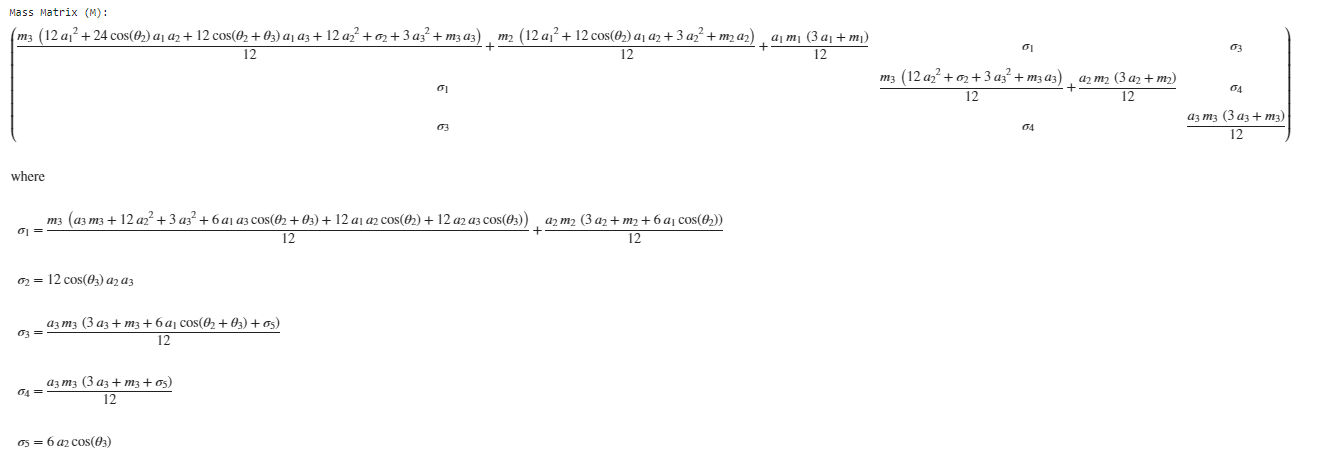
\includegraphics[width=1\linewidth]{../img/screenshot001}
	\caption{}
	\label{fig:screenshot001}
\end{figure}
\subsection*{ماتریس گرانش}
در گام بعد برای محاسبه ی ماتریس گرانش مطابق رابطه ی $5.65$ خواهیم داشت:
\[
\mathbf{g} = \begin{bmatrix} 0 \\ -g \\ 0 \end{bmatrix}
\]
\[
G_i = -m_i \mathbf{J}_{v_i}^T \mathbf{g}
\]
\[
G = \sum_{i=1}^{N} G_i = \sum_{i=1}^{N} \left( -m_i \mathbf{J}_{v_i}^T \mathbf{g} \right)
\]
با فراخوانی تابع
 $GravitationalVector$
  که بدین منظور نوشته شده است برای ربات $3R$ خواهیم داشت:
\[
\begin{array}{l}
	\left(\begin{array}{c}
		g\,m_3 \,{\left(\sigma_1 +a_1 \,\cos \left(\theta_1 \right)+\sigma_2 \right)}+g\,m_2 \,{\left(\frac{\sigma_1 }{2}+a_1 \,\cos \left(\theta_1 \right)\right)}+\frac{a_1 \,g\,m_1 \,\cos \left(\theta_1 \right)}{2}\\
		g\,m_3 \,{\left(\sigma_1 +\sigma_2 \right)}+\frac{a_2 \,g\,m_2 \,\cos \left(\theta_1 +\theta_2 \right)}{2}\\
		\frac{a_3 \,g\,m_3 \,\cos \left(\theta_1 +\theta_2 +\theta_3 \right)}{2}
	\end{array}\right)\\
	\mathrm{}\\
	\textrm{where}\\
	\mathrm{}\\
	\;\;\sigma_1 =a_2 \,\cos \left(\theta_1 +\theta_2 \right)\\
	\mathrm{}\\
	\;\;\sigma_2 =\frac{a_3 \,\cos \left(\theta_1 +\theta_2 +\theta_3 \right)}{2}
\end{array}
\]
\subsection*{ماتریس کوریولیس}
در ادامه، ماتریس کوریولیس مطابق روابط $5.34$ و $5.37$ محاسبه می شود. در این روابط داریم:
\[
\dot{M}(i,j) = \sum_{k=1}^{n} \frac{\partial M(i,j)}{\partial \theta_k} \cdot \dot{\theta}_k
\]
\begin{figure}[!h]
	\centering
	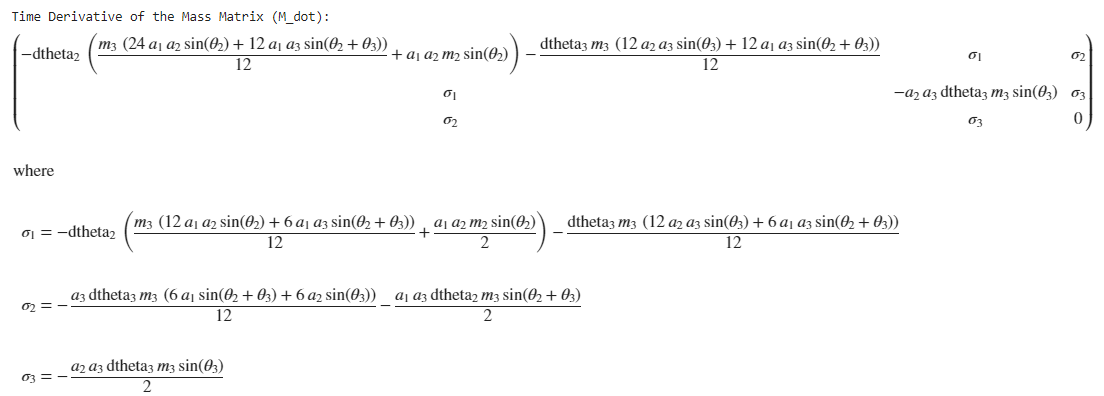
\includegraphics[width=1\linewidth]{../img/screenshot002}
	\caption{}
	\label{fig:screenshot002}
\end{figure}
\[
\mathbf{B} = \dot{M} \cdot \dot{\theta} - \frac{\partial K}{\partial \theta}
\]
\begin{figure}[!h]
	\centering
	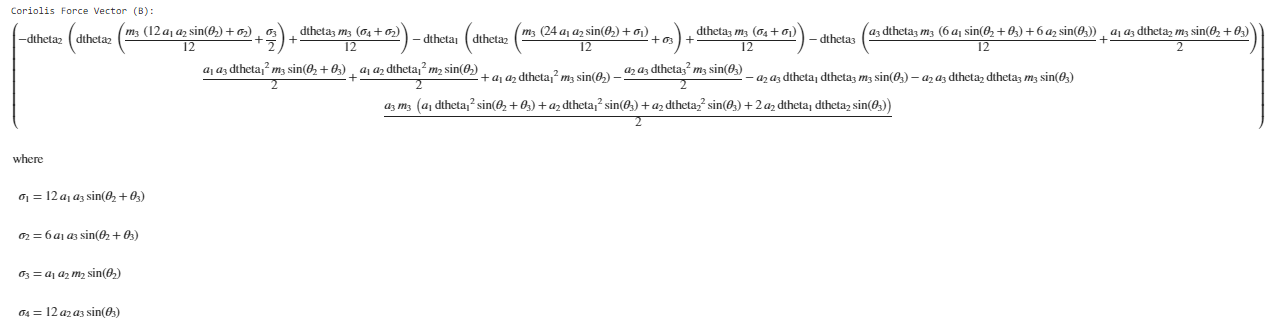
\includegraphics[width=1\linewidth]{../img/screenshot003}
	\caption{}
	\label{fig:screenshot003}
\end{figure}
\[
K = \frac{1}{2} \dot{\theta}^T M \dot{\theta}
\]
\section*{پاسخ سوال سه}
با استفاده از این روابط و توابع نوشته شده برای هر یک که در این برنامه با نام های $MassMatrixTimeDerivative$،
$CoriolisForceVector$
و 
$KineticEnergy$
تعریف شده اند، می توانیم ماتریس های مورد نظر را به دست بیاوریم که در اینجا از ذکر کردن نتایج تمامی مقادیر بالا به دلیل فضای ناکافی اجتناب شده است.

در نهایت، پس از تعریف هر یک از این ماتریس ها، می توانیم معادلات دینامیکی سیستم را طبق رابطه ی زیر به دست بیاوریم.
\[
Q = B(q, \dot{q}) + G(q) + M(q) \cdot \ddot{\theta}
\]
نتیجه ی این ماتریس در فایل متلب نمایش داده شده است.
\section*{پاسخ سوال چهار}
با اجرای برنامه به ازای تعداد درجات آزادی مختلف از 1 تا 7، تلاش می کنیم تا زمان اجرای برنامه را مقایسه کنیم. انتظار می رود که با توجه به حجم بالای محاسبات ماتریسی، با افزایش درجات آزادی زمان اجرای برنامه به صورت صعودی و نمایی افزایش یابد. برای این کار، از دستور $tic toc$ متلب استفاده شده است. مطابق آنچه که در تصویر زیر نمایش داده شده است، زمان های اجرای برنامه مشخص شده است. لازم به ذکر است که این فرایند بدون استفاده از حلقه ی for صورت گرفته و در نتیجه اعداد گزارش شده هر بار مجزا اندازه گیری شده است. علت این امر، نیاز به تغییر پارامترهای ورودی سیستم  از جمله پارامتر های DH بوده که به دلیل پیچیدگی زیاد، از آن صرف نظر شده است
\begin{figure}[!h]
	\centering
	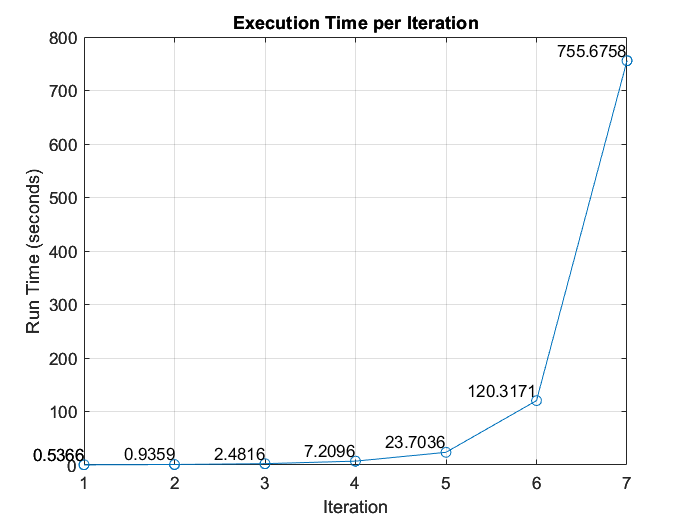
\includegraphics[width=1\linewidth]{../img/screenshot004}
	\caption{}
	\label{fig:screenshot004}
\end{figure}
\section*{پاسخ سوال پنج}
کسب اطمینان از صحت پاسخ های به دست آمده، همانطور که در متن سوال ذکر شده است به دو روش Verification به معنای تایید و Validation به معنای اعتبارسنجی انجام می گیرد که در ادامه به توضیح هر یک خواهیم پرداخت.
\subsection*{Verification}
منظور از تایید، آن است که مطمئن شویم محاسبات پیاده سازی شده با تئوری های موجود در این زمینه یکسان باشند. بنابراین، روش پیشنهادی برای تایید فرایند آن است که به صورت جز به جز محاسبات، فرمول ها و روابط مورد بررسی قرار بگیرند و در صورت بروز اشتباهات منطقی و یا محاسباتی رفع شوند. همچنین، در هر مرحله با استفاده از نمونه های ساده تر که قبلا درستی آنها اثبات شده است، می توان پاسخ های به دست آمده را با مقادیرر مرجع مقایسه کرد.
\subsection*{Validation}
اعتبارسنجی نتایح به دست آمده پس از تایید فرایند انجام می شود. در این تست، هدف آن است که مشخص شود پاسخ های به دست آمده از برنامه که صحت اجرا و محاسبات آنان به درستی انجام شده است، آیا در مثال های واقعی و کاربردی نیز صدق می کند یا خیر. برای این منظور، معمولا نتایج شبیه سازی و محاسبات با نسخه های واقعی از سیستم، نتایج گزارش شده در منابع معتبر نظیر مقالات و یا داده های معتبر مقایسه می شوند و در صورتی که مدل توانسته باشد به خوبی عمل کند، می توان انتظار داشت که نتایج به دست آمده از آن با منابع همخوانی داشته باشد

\section*{پاسخ سوال شش}
برای محاسبه دینامیک سیستم‌های رباتیکی، روش‌های متعددی وجود دارند که هر یک از نظر کارایی و هزینه محاسباتی متفاوت عمل می‌کنند. یکی از این روش‌ها، روش کلاسیک \textbf{اولر-لاگرانژ} است که از توابع انرژی برای استخراج معادلات حرکت استفاده می‌کند. اما با افزایش تعداد لینک‌های ربات، این روش به طور فزاینده‌ای محاسباتی و زمان‌بر می‌شود. به عنوان مثال، زمان اجرای این روش برای تعداد لینک‌های ۱ تا ۷ به ترتیب$0.533،$،$0.93$، $2.48$، $7.2$، $23$، $120$   و $750$ به دست آمده است.
	
روش‌های جایگزین دیگری نیز وجود دارند که از نظر هزینه محاسباتی عملکرد بهتری دارند:

	\begin{itemize}
		\item \textbf{روش نیوتن-اولر}:
این روش از قوانین نیوتن و اولر برای محاسبه نیروها و گشتاورها در هر لینک استفاده می‌کند و محاسبات را به صورت بازگشتی انجام می‌دهد. این ساختار بازگشتی باعث افزایش کارایی محاسبات می‌شود و نیاز به محاسبه و وارون‌سازی ماتریس‌های بزرگ که در روش اولر-لاگرانژ معمول است را حذف می‌کند.
		
		\item \textbf{الگوریتم‌های بازگشتی}:
الگوریتم‌هایی مانند \textbf{الگوریتم بدنه سخت ترکیبی (CRBA)} و \textbf{الگوریتم بدنه مفصل‌دار (ABA)} از روش‌های بازگشتی برای محاسبه دینامیک استفاده می‌کنند. این الگوریتم‌ها دارای پیچیدگی محاسباتی خطی هستند ($O(n)$) و این ویژگی باعث می‌شود که حتی با افزایش تعداد لینک‌ها، زمان محاسبات به صورت خطی افزایش یابد. این روش‌ها برای کاربردهای زمان واقعی بسیار مناسب هستند.
		
		\item \textbf{انتگرال‌گیرهای واریاسیونی}:
این روش‌ها از روش‌های عددی برای حفظ ویژگی‌های هندسی دینامیک سیستم، مانند انرژی و تکانه، استفاده می‌کنند. در سال‌های اخیر، پیشرفت‌هایی در این حوزه صورت گرفته است که منجر به توسعه انتگرال‌گیرهای واریاسیونی با پیچیدگی خطی برای سیستم‌های چندجسمی شده است. این روش‌ها دقت بالا و کارایی محاسباتی را ترکیب می‌کنند و برای شبیه‌سازی‌ها و بهینه‌سازی‌های مسیر بسیار مفید هستند.
	\end{itemize}
	
	با مقایسه این روش‌ها، می‌توان گفت:
	\begin{itemize}
		\item روش اولر-لاگرانژ با وجود ساختار منظم، در سیستم‌های پیچیده و با درجات آزادی بالا، هزینه محاسباتی بالایی دارد.
		\item روش نیوتن-اولر به دلیل ساختار بازگشتی خود، محاسبات را کارآمدتر انجام می‌دهد و برای کنترل زمان واقعی مناسب‌تر است.
		\item الگوریتم‌های بازگشتی مانند CRBA و ABA به دلیل پیچیدگی خطی، بهترین عملکرد را در سیستم‌های با تعداد لینک‌های زیاد ارائه می‌دهند.
		\item انتگرال‌گیرهای واریاسیونی ترکیبی از دقت و کارایی را ارائه می‌دهند و برای کاربردهایی که نیاز به حفظ ویژگی‌های هندسی دینامیک دارند، مناسب هستند.
	\end{itemize}











